\documentclass{beamer}

\usepackage[english]{babel}
\usepackage[utf8]{inputenc}

\usepackage{graphicx} % Immagini fantastiche e...
\graphicspath{        % dove trovarle
  {./images/},
  {../images/2D/},
  {../images/3D/},
  {../images/scratchpixel/},
}

%\usepackage{float}
%\usepackage{color}
%\usepackage{caption}
%\usepackage{subcaption}

%\usepackage{hyperref}
%\hypersetup{colorlinks=true, linkcolor=black, citecolor=black, plainpages=false, urlcolor=blue}
\usepackage{wallpaper}
%\usepackage{algpseudocode,algorithm,algorithmicx}

%\usepackage{amsthm}
%\usepackage{amssymb}
%\usepackage{amsmath}

%\usepackage{algpseudocode,algorithm,algorithmicx}

 
% ================================ %
%          Cose Personali          %
% ================================ %
\newcommand{\abs}[1]{\lvert #1 \lvert}
\newcommand{\norm}[1]{\lvert\lvert #1 \lvert\lvert}

\newcommand\N{\ensuremath{\mathbb{N}}}
\newcommand\R{\ensuremath{\mathbb{R}}}
\newcommand\Z{\ensuremath{\mathbb{Z}}}
\renewcommand\O{\ensuremath{\emptyset}}
\newcommand\Q{\ensuremath{\mathbb{Q}}}
\newcommand\C{\ensuremath{\mathbb{C}}}

\newcommand\E{\ensuremath{\mathbb{E}}}
\newcommand\T{\ensuremath{\mathbb{T}}}
\renewcommand\inf{\ensuremath{\infty}}

%\newtheorem{theorem}{Theorem}[section]
%\newtheorem{corollary}{Corollary}[theorem]
%\newtheorem{lemma}[theorem]{Lemma}
%\newtheorem{definition}{Definition}[section]

%\theoremstyle{definition}
%\newtheorem{defi}{Def.}[section]


%%Information to be included in the title page:
\title{3D Renderer of Implicit Surfaces}
\author{Tristano Munini}
%\date{6 aprile 2021}
%\institute{Overleaf}
  %\LARGE{\underline{\textbf{ANNO ACCADEMICO 2019-2020}}}\\
%\logo{
\includegraphics{polloPallido}}



% ================================ %
%            Il Documento          %
% ================================ %
\begin{document}

{
  \usebackgroundtemplate{
    \centering
    
\includegraphics[width=\paperwidth]{polloPallido}
  }
  \frame{\titlepage}
}

\begin{frame}
\frametitle{Index}
\begin{itemize}
  \item Signed Distance Functions
  \item Ray Tracing
    \begin{itemize}
      \item Rays and Cameras
      \item Sphere Tracing
      \item Lighting and Shadows
      \item Cone-Tracing
    \end{itemize}
  \item Implementation
\end{itemize}
\end{frame}

\begin{frame}
\frametitle{Signed Distance Functions : Distance Surfaces}
From \emph{``Sphere tracing: a geometric method for antialiased ray tracing of implicit surfaces"} an implicit surface is defined by a function that, given a point in space, indicates whether the point is inside, on or outside the surface.

\begin{definition}[Distance Surface]
A distance surface is implicitly defined by a function 
$f : \R^3 \to \R$ that characterizes $A \subset \R^3$, set of points that are on or inside the implicit surface:
$$ A = \{ x: f(x) \leq 0\} $$
\end{definition}

The surface can be also defined with $f^{-1}(0)$, which gives exactly the points on the surface.
\end{frame}

\begin{frame}
\frametitle{Signed Distance Functions : Point-To-Set Distance}
We can define the surface from the outside using a \emph{point-to-set} distance:
$$
d(x,A) = min_{y \in A} \norm{x - y}
$$
Thus $d(x,A)$, given a point $x \in \R^3$, returns the shortest distance to the surface defined by $A$.
\\
We can interchange $d(x,A)$ with $d(x, f^{-1}(0))$ even if they are slightly different, because here we'll handle points that aren't in surfaces interiors.
\end{frame}

\begin{frame}
\frametitle{Signed Distance Functions : Bound and SDF}
\begin{definition}[Signed Distance Bound]
We say that $f: \R^3 \to \R$ is a signed distance bound of its implicit surface $f^{-1}(0)$ if and only if
\begin{equation}\label{eq:sdb}
\abs{f(x)} \leq d(x,f^{-1}(0))
\end{equation}
\end{definition}

\begin{definition}[Signed Distance Function]
We say that $f$ is a signed distance function (SDF) when holds
\begin{equation}\label{eq:sdf}
\abs{f(x)} = d(x,f^{-1}(0))
\end{equation}
\end{definition}

The first definition says that a signed distance bound is always at least as cautious as the true distance function $d(x,f^{-1}(0))$ or the SDF.
\end{frame}

\begin{frame}
\frametitle{Signed Distance Functions : DUFs and DIFs}
Two other names for the concepts of the previous slide are
\emph{distance underestimate (implicit) functions} (DUFs) and 
\emph{distance implicit functions} (DIFs).

Remembering that $DUF(x) \leq DIF(x)$ for every DUFs and DIFs respecting the definitions above.

We will interchange Signed Distance Bound with DUF and SDF with DIF, because they express the same concepts.
\end{frame}


\begin{frame}
\frametitle{Signed Distance Functions : Lipschitz}
\begin{definition}[Lipschitz Function]
We say that a function $f : \R^3 \to \R$ is Lipschitz over a domain $D$ if and only if there is a positive, finite, constant $\lambda$ such that
\begin{equation}\label{eq:lip_fun}
\abs{f(x) - f(y)} \leq \lambda \norm{x - y}
\end{equation}
Such $\lambda$ is called the Lipschitz constant.
\end{definition}

There is no upper limit to $\lambda$, but there is a lower bound.
Let $Lip(f)$ be the function returning such minimum value.
\end{frame}


\begin{frame}
\frametitle{Signed Distance Functions : Lipschitz}
Manipulating \autoref{eq:lip_fun} we can observe that
\begin{align*}
  \lambda &\geq \dfrac{\abs{f(x) - f(y)}}{\norm{x - y}} \\
  \lambda &\geq \dfrac{f(x) - f(y)}{\norm{x - y}} \\ %\;\;\; \text{ remember $\lambda$ is positive } \\
  \lambda &\geq \lim_{\norm{x-y} \to 0} \dfrac{f(x) - f(y)}{x - y} = f'(x)
\end{align*}
the last step, given the continuity of $f$, permits us to estimate a safe lower bound for the Lipschitz constant.

\begin{theorem}
  Let $f$ be Lipschitz with Lipschitz constant $\lambda$.
  Then the function $f / \lambda$ is a SDF of its implicit surface.
\end{theorem}
\begin{proof}
  In the assignment.
\end{proof}
\end{frame}

\begin{frame}
\frametitle{Signed Distance Functions : Examples}

\begin{figure}[!htb]
\minipage{0.32\textwidth}
  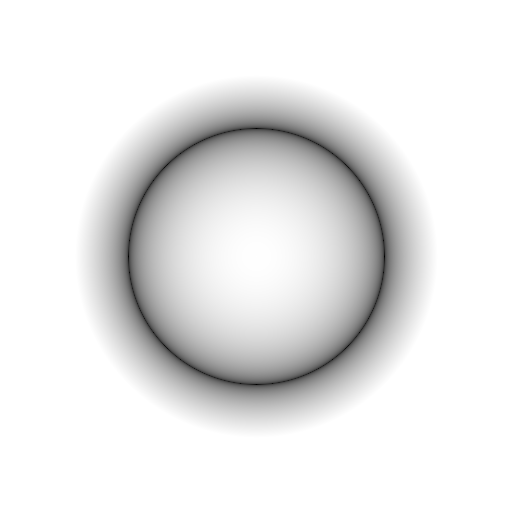
\includegraphics[width=\linewidth]{circle.png}
  %\caption{A circle}\label{fig:circle}
\endminipage\hfill
\minipage{0.32\textwidth}
  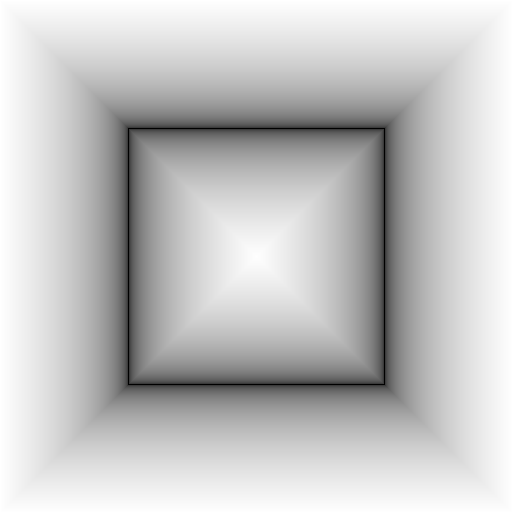
\includegraphics[width=\linewidth]{square.png}
  %\caption{A square}\label{fig:square}
\endminipage\hfill
\minipage{0.32\textwidth}%
  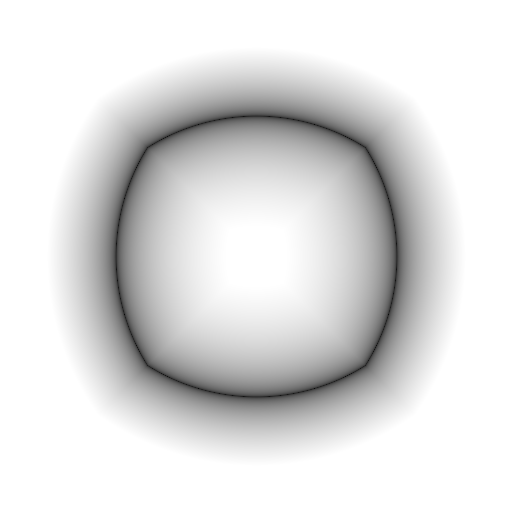
\includegraphics[width=\linewidth]{squircle.png}
  %\caption{A squircle}\label{fig:squircle}
\endminipage
\end{figure}

The images can be seen as 2D section of 3D objects done with a yz-aligned plane passing through the origin.
\begin{align*}
  \text{circle }  &: x^2 + y^2 - 1 \\
  \text{square }  &: max(\abs{x}, \abs{y}) - 1 \\
  \text{squircle }&: k * (max(\abs{x}, \abs{y}) - 1) + (1-k) * (x^2 + y^2 - 1)\\
                  &\;\;\;\;\;\;\text{where $k \in [0,1]$}
\end{align*}
\end{frame}


\begin{frame}
\frametitle{Signed Distance Functions : Constructive Solid Geometry}
SDFs make easy to create complex shapes from few simple primitives.
This technique it known as Constructive Solid Geometry (CSG).
\begin{itemize}
  \item union $ min(f_1, f_2) $
  \item intersection $ max(f_1, f_2) $
  \item subtraction $ max(f_1, -f_2) $
  \item mixing $ k*f_1 + (1-k) * f_2 \;\;\; \text{with $k\in[0,1]$} $
\end{itemize}
\end{frame}



\begin{frame}
\frametitle{Signed Distance Functions : Constructive Solid Geometry}
\begin{figure}[!htb]
  \centering
  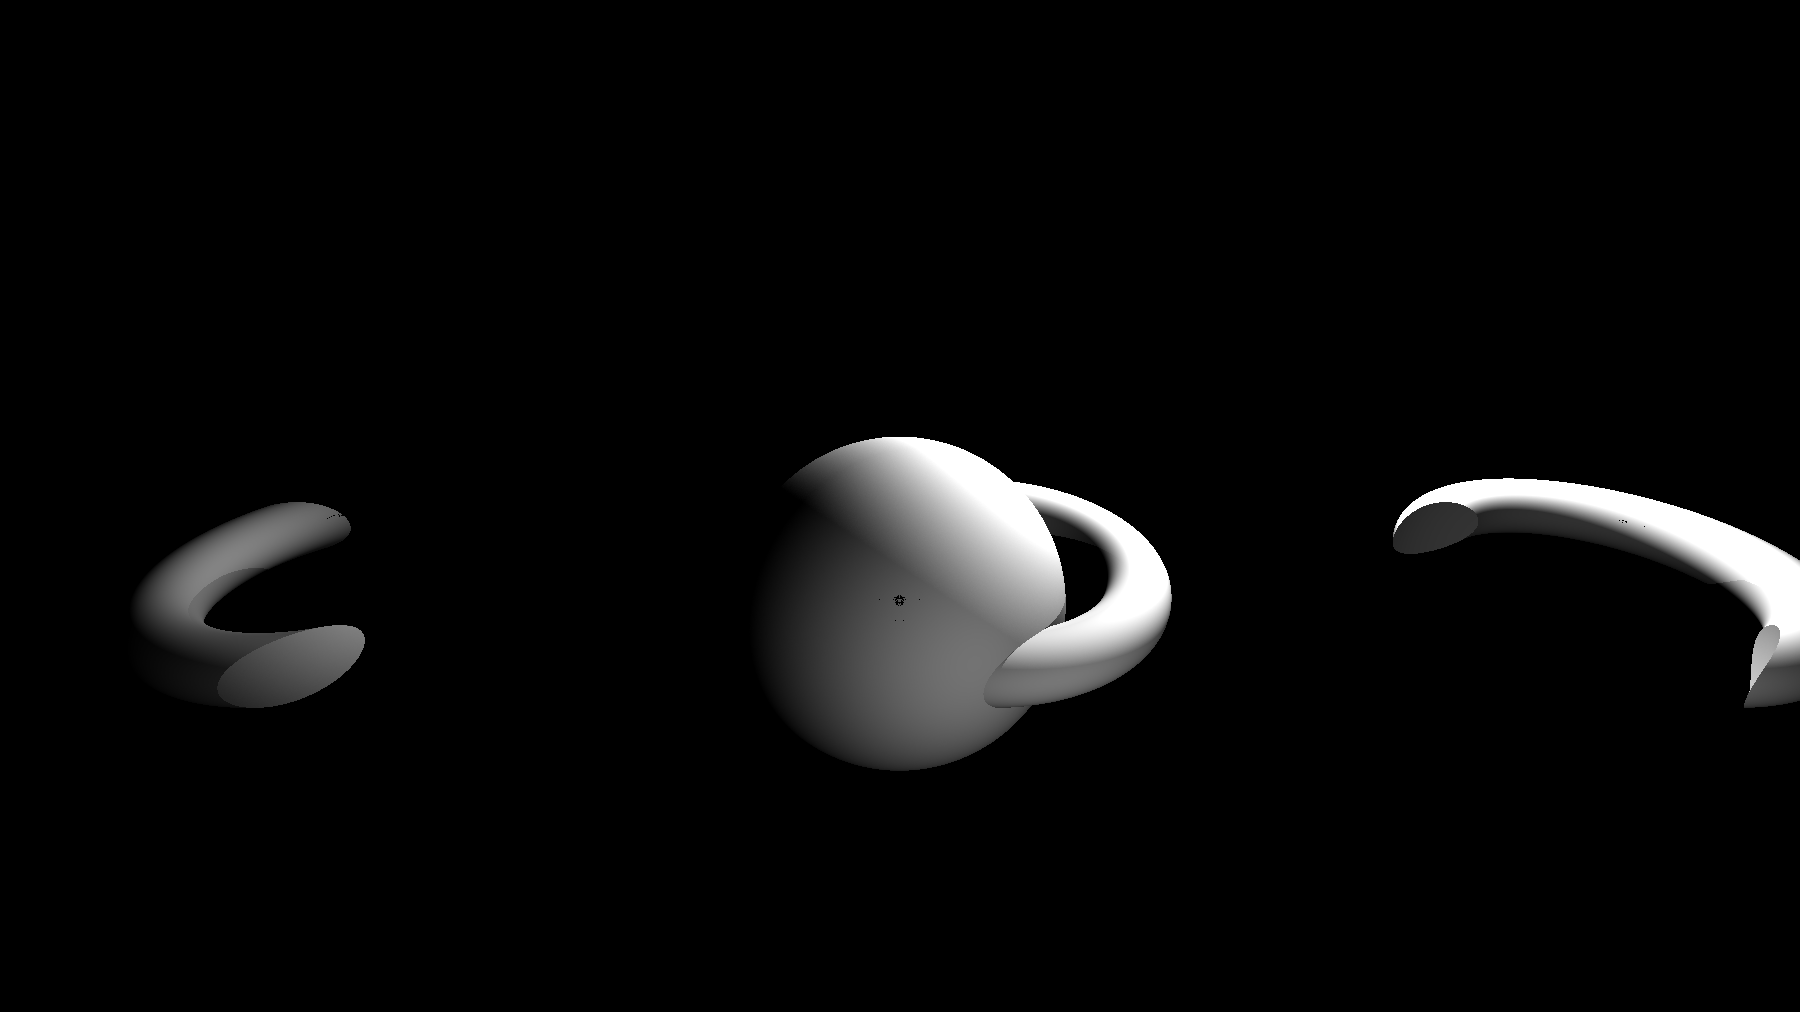
\includegraphics[width=\linewidth]{img_03.png}
\end{figure}
From left to right:
intersection, union and subtraction of a sphere and a torus.
\end{frame}

%%%%%%%%%%%%%%%%%%%%%%%%%%%%%%%%%%%%%%%%%%%%%%%%%%%%%%%%%%%%%%%%%%%%%%%%%%%%%%%%%%%%%%%%%%%%%%%
%% RAY TRACING
%%%%%%%%%%%%%%%%%%%%%%%%%%%%%%%%%%%%%%%%%%%%%%%%%%%%%%%%%%%%%%%%%%%%%%%%%%%%%%%%%%%%%%%%%%%%%%%

\begin{frame}
\frametitle{Ray Tracing : Rays and Cameras}

A ray is defined as a point and a direction in formulas:
$$
r(t) = O + tR
$$
where $O,R \in \R^3$ and $R$ is a unit vector.

At each time $t$ we can compute a point position on the ray.
\begin{figure}[!htb]
  \centering
  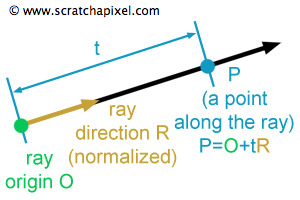
\includegraphics[width=.5\linewidth]{ray.png}
\end{figure}
\end{frame}


\begin{frame}
\frametitle{Ray Tracing : Rays and Cameras}
\begin{figure}[!htb]
  \centering
  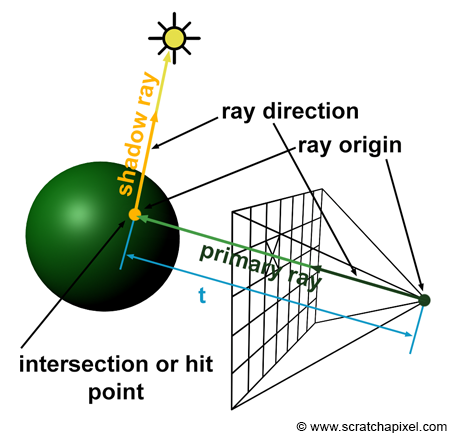
\includegraphics[width=.5\linewidth]{pinhole_camera.png}
\end{figure}
A pinhole camera inside a scene with a sphere and a light source.
\end{frame}
% QUA SI POTREBBE PARLARE DI PIU' DELLA CAMERA MA DIPENDE DA TEMPO E SPAZIO

\begin{frame}
\frametitle{Ray Tracing : Sphere Tracing}
Ray Marching proceeds along the rays with a fixed step, with sphere tracing an adaptive step is used.


\end{frame}






















%\begin{frame}
%\frametitle{Example}
%\begin{figure}[ht]
%  \includegraphics[width=\textwidth]{example-image-a}
%\end{figure}
%\end{frame}

\end{document}
